\documentclass[border=8pt]{standalone}
\usepackage[T1]{fontenc}\usepackage{helvet}\renewcommand{\familydefault}{\sfdefault}
\usepackage{tikz}\usetikzlibrary{arrows.meta, positioning, calc, backgrounds}
\definecolor{ink}{HTML}{1a1916}
\definecolor{inktwo}{HTML}{3a3a35}
\definecolor{inkthree}{HTML}{6a6862}
\definecolor{rule}{HTML}{b8b09a}
\definecolor{amber}{HTML}{a8730a}
\definecolor{red}{HTML}{c8261a}
\definecolor{paper}{HTML}{f0eee5}
\definecolor{slab}{HTML}{d8d4c6}
\tikzset{
  >={Stealth[length=2.2mm]},
  wire/.style={line width=0.8pt, ink},
  modwire/.style={line width=0.6pt, dashed, ink},
  tastewire/.style={line width=0.6pt, dashed, amber},
  gatewire/.style={line width=0.6pt, dotted, ink},
  block/.style={rectangle, draw=ink, line width=0.9pt, fill=slab, minimum width=3.0cm, minimum height=1.9cm, inner sep=0pt},
  perf/.style={rectangle, draw=ink, line width=0.7pt, minimum width=3.0cm, minimum height=0.7cm, inner sep=2pt, font=\footnotesize, text=ink},
  title/.style={font=\scriptsize\bfseries, text=ink, anchor=north, inner sep=2pt},
  jack/.style={circle, draw=ink, fill=paper, line width=0.5pt, minimum size=3.2pt, inner sep=0pt},
  plabel/.style={font=\tiny, text=inktwo, anchor=west, inner sep=1pt},
  olabel/.style={font=\tiny, text=inktwo, anchor=east, inner sep=1pt},
  settings/.style={font=\scriptsize, text=ink, align=left, anchor=north west, inner sep=1pt, text width=2.9cm},
}
\begin{document}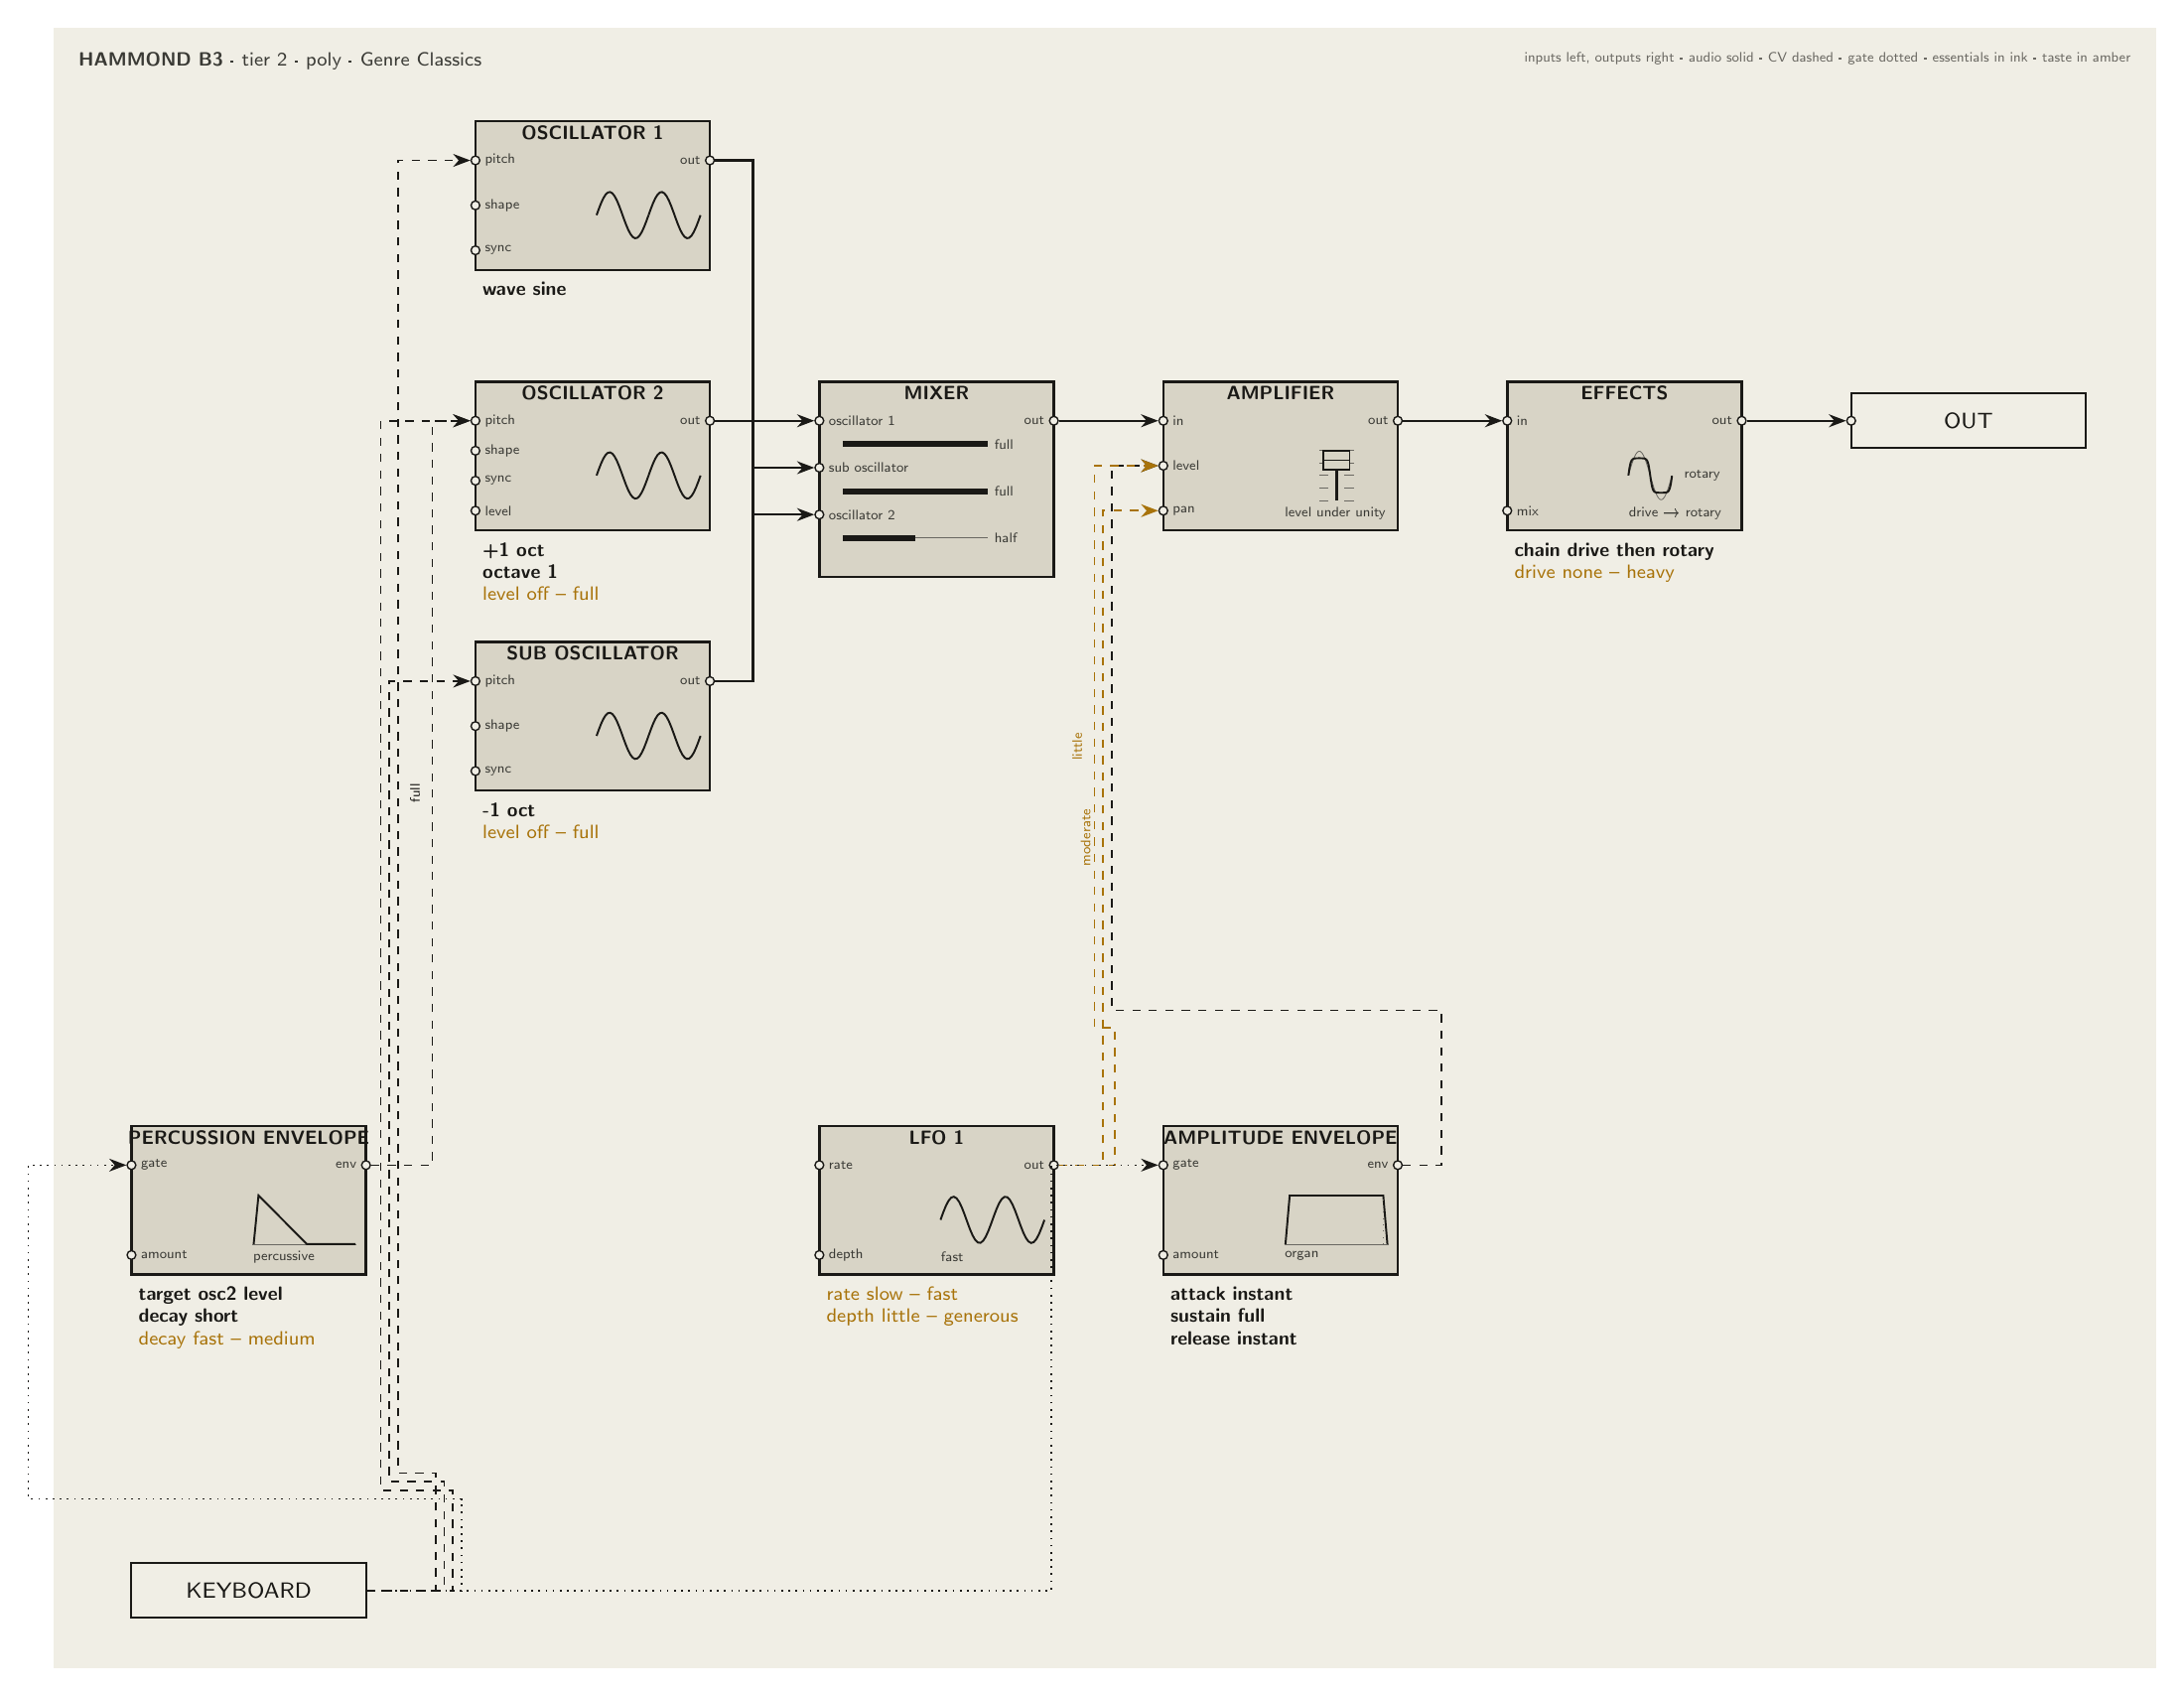
\begin{tikzpicture}
\begin{scope}[on background layer]\fill[paper] (-2.5,-15.509999999999998) rectangle (24.4,5.48);\end{scope}
\node[block, minimum height=1.9cm] (osc1) at (4.4,3.33) {};
\node[title] at (osc1.north) {OSCILLATOR 1};
\node[jack] (osc1-pitch) at (2.9000000000000004,3.7800000000000002) {};
\node[plabel] at (2.9800000000000004,3.7800000000000002) {pitch};
\node[jack] (osc1-shape) at (2.9000000000000004,3.205) {};
\node[plabel] at (2.9800000000000004,3.205) {shape};
\node[jack] (osc1-sync) at (2.9000000000000004,2.6300000000000003) {};
\node[plabel] at (2.9800000000000004,2.6300000000000003) {sync};
\node[jack] (osc1-out) at (5.9,3.7800000000000002) {};
\node[olabel] at (5.82,3.7800000000000002) {out};
\begin{scope}
\draw[ink, line width=0.7pt] plot[domain=0.000:0.500, samples=24, variable=\u] ({4.450+\u*1.330},{2.710+(0.740)*(0.5+0.4*sin(360*(\u*2))+0.0)});
\draw[ink, line width=0.7pt] plot[domain=0.500:1.000, samples=24, variable=\u] ({4.450+\u*1.330},{2.710+(0.740)*(0.5+0.4*sin(360*(\u*2))+0.0)});
\end{scope}
\node[settings] at (2.95,2.26) {\textbf{wave sine}};
\node[block, minimum height=1.9cm] (osc2) at (4.4,0.0) {};
\node[title] at (osc2.north) {OSCILLATOR 2};
\node[jack] (osc2-pitch) at (2.9000000000000004,0.44999999999999996) {};
\node[plabel] at (2.9800000000000004,0.44999999999999996) {pitch};
\node[jack] (osc2-shape) at (2.9000000000000004,0.06666666666666665) {};
\node[plabel] at (2.9800000000000004,0.06666666666666665) {shape};
\node[jack] (osc2-sync) at (2.9000000000000004,-0.31666666666666665) {};
\node[plabel] at (2.9800000000000004,-0.31666666666666665) {sync};
\node[jack] (osc2-level) at (2.9000000000000004,-0.7) {};
\node[plabel] at (2.9800000000000004,-0.7) {level};
\node[jack] (osc2-out) at (5.9,0.44999999999999996) {};
\node[olabel] at (5.82,0.44999999999999996) {out};
\begin{scope}
\draw[ink, line width=0.7pt] plot[domain=0.000:0.500, samples=24, variable=\u] ({4.450+\u*1.330},{-0.620+(0.740)*(0.5+0.4*sin(360*(\u*2))+0.0)});
\draw[ink, line width=0.7pt] plot[domain=0.500:1.000, samples=24, variable=\u] ({4.450+\u*1.330},{-0.620+(0.740)*(0.5+0.4*sin(360*(\u*2))+0.0)});
\end{scope}
\node[settings] at (2.95,-1.0699999999999998) {\textbf{+1 oct} \\ \textbf{octave 1} \\ \textcolor{amber}{level off -- full}};
\node[block, minimum height=1.9cm] (sub) at (4.4,-3.33) {};
\node[title] at (sub.north) {SUB OSCILLATOR};
\node[jack] (sub-pitch) at (2.9000000000000004,-2.88) {};
\node[plabel] at (2.9800000000000004,-2.88) {pitch};
\node[jack] (sub-shape) at (2.9000000000000004,-3.455) {};
\node[plabel] at (2.9800000000000004,-3.455) {shape};
\node[jack] (sub-sync) at (2.9000000000000004,-4.029999999999999) {};
\node[plabel] at (2.9800000000000004,-4.029999999999999) {sync};
\node[jack] (sub-out) at (5.9,-2.88) {};
\node[olabel] at (5.82,-2.88) {out};
\begin{scope}
\draw[ink, line width=0.7pt] plot[domain=0.000:0.500, samples=24, variable=\u] ({4.450+\u*1.330},{-3.950+(0.740)*(0.5+0.4*sin(360*(\u*2))+0.0)});
\draw[ink, line width=0.7pt] plot[domain=0.500:1.000, samples=24, variable=\u] ({4.450+\u*1.330},{-3.950+(0.740)*(0.5+0.4*sin(360*(\u*2))+0.0)});
\end{scope}
\node[settings] at (2.95,-4.4) {\textbf{-1 oct} \\ \textcolor{amber}{level off -- full}};
\node[block, minimum height=2.5cm] (mix) at (8.8,-0.30000000000000004) {};
\node[title] at (mix.north) {MIXER};
\node[jack] (mix-osc1) at (7.300000000000001,0.44999999999999996) {};
\node[plabel] at (7.380000000000001,0.44999999999999996) {oscillator 1};
\draw[inkthree, line width=0.3pt] (7.600,0.150) -- (9.450,0.150);
\draw[ink, line width=2.2pt] (7.600,0.150) -- (9.450,0.150);
\node[font=\tiny, text=inktwo, anchor=west, inner sep=1pt] at (9.500,0.150) {full};
\node[jack] (mix-sub) at (7.300000000000001,-0.15000000000000002) {};
\node[plabel] at (7.380000000000001,-0.15000000000000002) {sub oscillator};
\draw[inkthree, line width=0.3pt] (7.600,-0.450) -- (9.450,-0.450);
\draw[ink, line width=2.2pt] (7.600,-0.450) -- (9.450,-0.450);
\node[font=\tiny, text=inktwo, anchor=west, inner sep=1pt] at (9.500,-0.450) {full};
\node[jack] (mix-osc2) at (7.300000000000001,-0.75) {};
\node[plabel] at (7.380000000000001,-0.75) {oscillator 2};
\draw[inkthree, line width=0.3pt] (7.600,-1.050) -- (9.450,-1.050);
\draw[ink, line width=2.2pt] (7.600,-1.050) -- (8.525,-1.050);
\node[font=\tiny, text=inktwo, anchor=west, inner sep=1pt] at (9.500,-1.050) {half};
\node[jack] (mix-out) at (10.3,0.44999999999999996) {};
\node[olabel] at (10.22,0.44999999999999996) {out};
\node[block, minimum height=1.9cm] (amp) at (13.200000000000001,0.0) {};
\node[title] at (amp.north) {AMPLIFIER};
\node[jack] (amp-in) at (11.700000000000001,0.44999999999999996) {};
\node[plabel] at (11.780000000000001,0.44999999999999996) {in};
\node[jack] (amp-level) at (11.700000000000001,-0.125) {};
\node[plabel] at (11.780000000000001,-0.125) {level};
\node[jack] (amp-pan) at (11.700000000000001,-0.7) {};
\node[plabel] at (11.780000000000001,-0.7) {pan};
\node[jack] (amp-out) at (14.700000000000001,0.44999999999999996) {};
\node[olabel] at (14.620000000000001,0.44999999999999996) {out};
\begin{scope}
\draw[ink, line width=1.2pt] (13.915,-0.570) -- (13.915,0.070);
\draw[inkthree, line width=0.3pt] (13.695,-0.570) -- (13.815,-0.570) (14.015,-0.570) -- (14.135,-0.570);
\draw[inkthree, line width=0.3pt] (13.695,-0.410) -- (13.815,-0.410) (14.015,-0.410) -- (14.135,-0.410);
\draw[inkthree, line width=0.3pt] (13.695,-0.250) -- (13.815,-0.250) (14.015,-0.250) -- (14.135,-0.250);
\draw[inkthree, line width=0.3pt] (13.695,-0.090) -- (13.815,-0.090) (14.015,-0.090) -- (14.135,-0.090);
\draw[inkthree, line width=0.3pt] (13.695,0.070) -- (13.815,0.070) (14.015,0.070) -- (14.135,0.070);
\fill[slab, draw=ink, line width=0.6pt] (13.745,-0.178) rectangle (14.085,0.062);
\draw[ink, line width=0.5pt] (13.745,-0.058) -- (14.085,-0.058);
\node[font=\tiny, text=inktwo, anchor=north west, inner sep=0pt] at (13.250,-0.650) {level under unity};
\end{scope}
\node[block, minimum height=1.9cm] (fx) at (17.6,0.0) {};
\node[title] at (fx.north) {EFFECTS};
\node[jack] (fx-in) at (16.1,0.44999999999999996) {};
\node[plabel] at (16.18,0.44999999999999996) {in};
\node[jack] (fx-mix) at (16.1,-0.7) {};
\node[plabel] at (16.18,-0.7) {mix};
\node[jack] (fx-out) at (19.1,0.44999999999999996) {};
\node[olabel] at (19.020000000000003,0.44999999999999996) {out};
\begin{scope}
\draw[inkthree, line width=0.3pt] plot[domain=0.000:0.420, samples=30, variable=\u] ({17.650+\u*1.330},{-0.620+(0.740)*(0.5+0.42*sin(360*((\u-0.000)/0.420)))});
\draw[ink, line width=0.7pt] plot[domain=0.000:0.420, samples=40, variable=\u] ({17.650+\u*1.330},{-0.620+(0.740)*(0.5+0.3*tanh(3*sin(360*((\u-0.000)/0.420))))});
\node[font=\tiny, text=inktwo] at (18.594,-0.250) {rotary};
\node[font=\tiny, text=inktwo, anchor=north west, inner sep=0pt] at (17.650,-0.650) {drive → rotary};
\end{scope}
\node[settings] at (16.150000000000002,-1.0699999999999998) {\textbf{chain drive then rotary} \\ \textcolor{amber}{drive none -- heavy}};
\node[block, minimum height=1.9cm] (menv) at (0.0,-9.52) {};
\node[title] at (menv.north) {PERCUSSION ENVELOPE};
\node[jack] (menv-gate) at (-1.5,-9.07) {};
\node[plabel] at (-1.42,-9.07) {gate};
\node[jack] (menv-amount) at (-1.5,-10.22) {};
\node[plabel] at (-1.42,-10.22) {amount};
\node[jack] (menv-out) at (1.5,-9.07) {};
\node[olabel] at (1.42,-9.07) {env};
\begin{scope}
\draw[inkthree, line width=0.3pt] (0.050,-10.081) -- (1.380,-10.081);
\draw[ink, line width=0.7pt] (0.063,-10.081) -- (0.125,-9.459) -- (0.746,-10.081) -- (0.746,-10.081) -- (1.367,-10.081);
\node[font=\tiny, text=inktwo, anchor=north west, inner sep=0pt] at (0.050,-10.170) {percussive};
\end{scope}
\node[settings] at (-1.45,-10.589999999999998) {\textbf{target osc2 level} \\ \textbf{decay short} \\ \textcolor{amber}{decay fast -- medium}};
\node[block, minimum height=1.9cm] (lfo1) at (8.8,-9.52) {};
\node[title] at (lfo1.north) {LFO 1};
\node[jack] (lfo1-rate) at (7.300000000000001,-9.07) {};
\node[plabel] at (7.380000000000001,-9.07) {rate};
\node[jack] (lfo1-depth) at (7.300000000000001,-10.22) {};
\node[plabel] at (7.380000000000001,-10.22) {depth};
\node[jack] (lfo1-out) at (10.3,-9.07) {};
\node[olabel] at (10.22,-9.07) {out};
\begin{scope}
\draw[ink, line width=0.7pt] plot[domain=0:1, samples=40, variable=\u] ({8.850+\u*1.330},{-10.140+(0.740)*(0.5+0.4*sin(360*\u*2))});
\node[font=\tiny, text=inktwo, anchor=north west, inner sep=0pt] at (8.850,-10.170) {fast};
\end{scope}
\node[settings] at (7.3500000000000005,-10.589999999999998) {\textcolor{amber}{rate slow -- fast} \\ \textcolor{amber}{depth little -- generous}};
\node[block, minimum height=1.9cm] (aenv) at (13.200000000000001,-9.52) {};
\node[title] at (aenv.north) {AMPLITUDE ENVELOPE};
\node[jack] (aenv-gate) at (11.700000000000001,-9.07) {};
\node[plabel] at (11.780000000000001,-9.07) {gate};
\node[jack] (aenv-amount) at (11.700000000000001,-10.22) {};
\node[plabel] at (11.780000000000001,-10.22) {amount};
\node[jack] (aenv-out) at (14.700000000000001,-9.07) {};
\node[olabel] at (14.620000000000001,-9.07) {env};
\begin{scope}
\draw[inkthree, line width=0.3pt] (13.250,-10.081) -- (14.580,-10.081);
\draw[ink, line width=0.7pt] (13.263,-10.081) -- (13.317,-9.459) -- (13.849,-9.459) -- (14.514,-9.459) -- (14.567,-10.081);
\draw[inkthree, line width=0.3pt, dotted] (14.514,-10.081) -- (14.514,-9.459);
\node[font=\tiny, text=inktwo, anchor=north west, inner sep=0pt] at (13.250,-10.170) {organ};
\end{scope}
\node[settings] at (11.750000000000002,-10.589999999999998) {\textbf{attack instant} \\ \textbf{sustain full} \\ \textbf{release instant}};
\node[perf] (key) at (0.0,-14.509999999999998) {KEYBOARD};
\node[perf, fill=paper] (out) at (22.0,0.44999999999999996) {OUT}; \node[jack] (out-in) at (20.5,0.44999999999999996) {};
\draw[wire,->] (osc1-out) -- (6.45,3.7800000000000002) |- (mix-osc1);
\draw[wire,->] (sub-out) -- (6.45,-2.88) |- (mix-sub);
\draw[wire,->] (osc2-out) -- (6.45,0.44999999999999996) |- (mix-osc2);
\draw[wire,->] (mix-out) -- (10.850000000000001,0.44999999999999996) |- (amp-in);
\draw[wire,->] (amp-out) -- (fx-in);
\draw[wire,->] (fx-out) -- (out-in);
\draw[modwire,->] (menv-out) -- (2.3500000000000005,-9.07) -- (2.3500000000000005,0.44999999999999996) -- (osc2-pitch);
\node[font=\tiny, text=ink, anchor=south, inner sep=1pt, rotate=90] at (2.2300000000000004,-4.3100000000000005) {full};
\draw[modwire,->] (aenv-out) -- (15.26,-9.07) -- (15.26,-7.090000000000001) -- (11.040000000000001,-7.090000000000001) -- (11.040000000000001,-0.125) -- (amp-level);
\draw[tastewire,->] (lfo1-out) -- (10.93,-9.07) -- (10.93,-0.7) -- (amp-pan);
\node[font=\tiny, text=amber, anchor=south, inner sep=1pt, rotate=90] at (10.81,-4.885) {moderate};
\draw[tastewire,->] (lfo1-out) -- (11.08,-9.07) -- (11.08,-7.3100000000000005) -- (10.82,-7.3100000000000005) -- (10.82,-0.125) -- (amp-level);
\node[font=\tiny, text=amber, anchor=south, inner sep=1pt, rotate=90] at (10.700000000000001,-3.7175000000000002) {little};
\draw[modwire,->] (key.east) -- (2.39,-14.509999999999998) -- (2.39,-13.009999999999998) -- (1.9100000000000006,-13.009999999999998) -- (1.9100000000000006,3.7800000000000002) -- (osc1-pitch);
\draw[modwire,->] (key.east) -- (2.5,-14.509999999999998) -- (2.5,-13.12) -- (1.8000000000000005,-13.12) -- (1.8000000000000005,-2.88) -- (sub-pitch);
\draw[modwire,->] (key.east) -- (2.61,-14.509999999999998) -- (2.61,-13.229999999999999) -- (1.6900000000000004,-13.229999999999999) -- (1.6900000000000004,0.44999999999999996) -- (osc2-pitch);
\draw[gatewire,->] (key.east) -- (2.7199999999999998,-14.509999999999998) -- (2.7199999999999998,-13.339999999999998) -- (-2.82,-13.339999999999998) -- (-2.82,-9.07) -- (menv-gate);
\draw[gatewire,->] (key.east) -- (10.27,-14.509999999999998) -- (10.27,-9.07) -- (aenv-gate);
\node[anchor=north west, font=\scriptsize, text=inktwo] at (-2.3,5.28) {\textbf{HAMMOND B3} · tier 2 · poly · Genre Classics};
\node[anchor=north east, font=\tiny, text=inkthree] at (24.2,5.28) {inputs left, outputs right · audio solid · CV dashed · gate dotted · essentials in ink · taste in amber};
\end{tikzpicture}\end{document}
